
%(BEGIN_QUESTION)
% Copyright 2010, Tony R. Kuphaldt, released under the Creative Commons Attribution License (v 1.0)
% This means you may do almost anything with this work of mine, so long as you give me proper credit

Suppose a 75 horsepower electric motor powered by three-phase 480 VAC power is used to turn a pump:

$$\includegraphics[width=15.5cm]{i04249x01.eps}$$

Using the conversion factor of 746 watts to one horsepower, calculate the amount of AC line current drawn by the motor at full power (assuming perfect efficiency).  

\vskip 10pt

If the motor were only 92\% efficient (92\% of the applied power performing mechanical work, and 8\% of the applied power wasted in the form of heat), how much AC current would it draw at full power then?

\vskip 10pt

Program a computer spreadsheet (e.g. Microsoft Excel) to calculate the same ideal and real current values requested above.  Build the spreadsheet page so that all the given values in this problem (75 HP, 480 VAC, and 92\% motor efficiency) may be edited by the user, allowing the spreadsheet to be used to calculate ideal and real motor currents for a variety of different motor scenarios.

\underbar{file i04249}
%(END_QUESTION)





%(BEGIN_ANSWER)

$I_{line}$ = 67.30 amps of current (assuming 100\% efficiency).

\vskip 10pt

$I_{line}$ = 73.15 amps of current (assuming 92\% efficiency).

%(END_ANSWER)





%(BEGIN_NOTES)

$$\left(75 \hbox{ HP} \over 1 \right) \left(746 \hbox{ W} \over 1 \hbox{ HP} \right) = 55950 \hbox{ W}$$

$$P = I V \sqrt{3}$$

$$I = {P \over {V \sqrt{3}}}$$

$$I = {55950 \hbox{ W} \over {480 \hbox{ V} \sqrt{3}}}$$

$$I = 67.30 \hbox{ A}$$

This calculation, of course, assumes 100\% efficiency.  If the motor is only 92\% efficient, it means the 75 HP of mechanical power is only 92\% of the electrical power input to the motor:

$$P_{out} = \eta P_{in}$$

$$P_{in} = {P_{out} \over \eta}$$

$$P_{in} = {55950 \hbox{ W} \over 0.92}$$

$$P_{in} = 60815 \hbox{ W}$$

Now that we know the input power for a 92\% efficient motor, we may calculate the motor current at 480 volts:

$$P = I V \sqrt{3}$$

$$I = {P \over {V \sqrt{3}}}$$

$$I = {60815 \hbox{ W} \over {480 \hbox{ V} \sqrt{3}}}$$

$$I = 73.15 \hbox{ A}$$


%INDEX% Electronics review: AC motor horsepower calculation (three-phase)

%(END_NOTES)

